% shared preamble of the theory figures (white background, purple / black theme, sans-serif)
\documentclass[tikz,border=8pt]{standalone}
\usepackage[T1]{fontenc}
\usepackage[scaled=0.92]{helvet}
\renewcommand{\familydefault}{\sfdefault}
\usepackage{amsmath,amssymb}
\usepackage[helvet]{sfmath}
\usetikzlibrary{arrows.meta,calc,decorations.pathreplacing,positioning,backgrounds}
\definecolor{ink}{HTML}{1A1A1F}
\definecolor{cohesin}{HTML}{6A3DE8}
\definecolor{condensin}{HTML}{1BAF7A}
\definecolor{fwd}{HTML}{D1303F}      % CTCF pointing right
\definecolor{rev}{HTML}{2B62D9}      % CTCF pointing left
\definecolor{panel}{HTML}{F8F6FD}
\definecolor{panelline}{HTML}{E3DDF5}
\tikzset{
  fiber/.style={line width=2.1pt,ink,line cap=round,line join=round},
  halo/.style={line width=6pt,white,line cap=round},
  lab/.style={font=\small,text=ink},
  note/.style={font=\footnotesize,text=ink!60},
  hd/.style={font=\bfseries\small,text=ink,anchor=west},
  leader/.style={line width=0.6pt,ink!45},
}
% soft panel, numbered badge, heading
\newcommand{\panelbg}[4]{\draw[rounded corners=9pt,fill=panel,draw=panelline,line width=0.9pt] (#1,#2) rectangle (#3,#4);}
\newcommand{\badge}[3]{\fill[ink] (#1,#2) circle (0.21);\node[white,font=\bfseries\footnotesize] at (#1,#2) {#3};}
% CTCF: a protein on the fibre carrying an arrow that gives the motif direction (f = right, r = left)
\newcommand{\protf}[2]{\draw[rounded corners=3.5pt,line width=0.6pt,draw=fwd!65!black,fill=fwd] (#1-0.3,#2-0.19) rectangle (#1+0.3,#2+0.19);
  \draw[white,line width=1.5pt,-{Stealth[length=3.4pt,width=4.4pt]}] (#1-0.15,#2)--(#1+0.16,#2);}
\newcommand{\protr}[2]{\draw[rounded corners=3.5pt,line width=0.6pt,draw=rev!65!black,fill=rev] (#1-0.3,#2-0.19) rectangle (#1+0.3,#2+0.19);
  \draw[white,line width=1.5pt,-{Stealth[length=3.4pt,width=4.4pt]}] (#1+0.15,#2)--(#1-0.16,#2);}
\newcommand{\prot}[3]{\csname prot#3\endcsname{#1}{#2}}
% ring seen at an angle, drawn as a tube (dark outline, light core); back half and front half
\newcommand{\ringpart}[5]{\draw[line width=4.6pt,#3!80!black,line cap=round] ([shift={(#1,#2)}]#4:0.55 and 0.21) arc[start angle=#4,end angle=#5,x radius=0.55,y radius=0.21];
  \draw[line width=2.4pt,#3!55!white,line cap=round] ([shift={(#1,#2)}]#4:0.55 and 0.21) arc[start angle=#4,end angle=#5,x radius=0.55,y radius=0.21];}
\newcommand{\ringback}[3]{\ringpart{#1}{#2}{#3}{180}{0}}
\newcommand{\ringfront}[3]{\ringpart{#1}{#2}{#3}{180}{360}}
% smooth loop whose foot (ring) is at (cx,y0): half-width W, height H, ring colour
\newcommand{\lloop}[5]{%
  \ringback{#1}{#2}{#5}%
  \draw[fiber] (#1-0.3,#2) .. controls (#1-0.3,#2+0.25*#4) and (#1-#3,#2+0.2*#4) .. (#1-#3,#2+0.55*#4)
     .. controls (#1-#3,#2+0.95*#4) and (#1-0.5*#3,#2+#4) .. (#1,#2+#4)
     .. controls (#1+0.5*#3,#2+#4) and (#1+#3,#2+0.95*#4) .. (#1+#3,#2+0.55*#4)
     .. controls (#1+#3,#2+0.2*#4) and (#1+0.3,#2+0.25*#4) .. (#1+0.3,#2);%
  \ringfront{#1}{#2}{#5}}
% gently undulating fibre from x0 to the loop foot at cx (height y0), and from x1
\newcommand{\base}[4]{%
  \draw[fiber] plot[smooth] coordinates {(#1,0.05) (#1+0.35*#3-0.35*#1,-0.05) (#3-1.4,0.04)} .. controls (#3-0.6,0.02) and (#3-0.3,0.05) .. (#3-0.3,#4);
  \draw[fiber] plot[smooth] coordinates {(#2,-0.05) (#2-0.35*#2+0.35*#3,0.05) (#3+1.4,-0.04)} .. controls (#3+0.6,-0.02) and (#3+0.3,0.05) .. (#3+0.3,#4);}
% stop sign for a blocked leg and a leg arrow
\newcommand{\stopbar}[3]{\draw[#3,line width=2.4pt,line cap=round] (#1,#2-0.2)--(#1,#2+0.2);}
\newcommand{\legarrow}[3]{\draw[cohesin,line width=1.6pt,-{Stealth[length=5pt,width=6pt]},line cap=round] (#1,#3)--(#2,#3);}

\definecolor{A}{HTML}{D1303F}\definecolor{B}{HTML}{5B4FD6}
\tikzset{ln/.style={line width=0.7pt,ink!45},cur/.style={line width=1.8pt,cohesin},thin/.style={line width=0.9pt},
  mv/.style={line width=1.2pt,ink!70,-{Stealth[length=5pt,width=6pt]}},box/.style={rounded corners=5pt,draw=cohesin!70,fill=white,line width=0.9pt,align=center,font=\small,text=ink,inner sep=4pt}}
\begin{document}
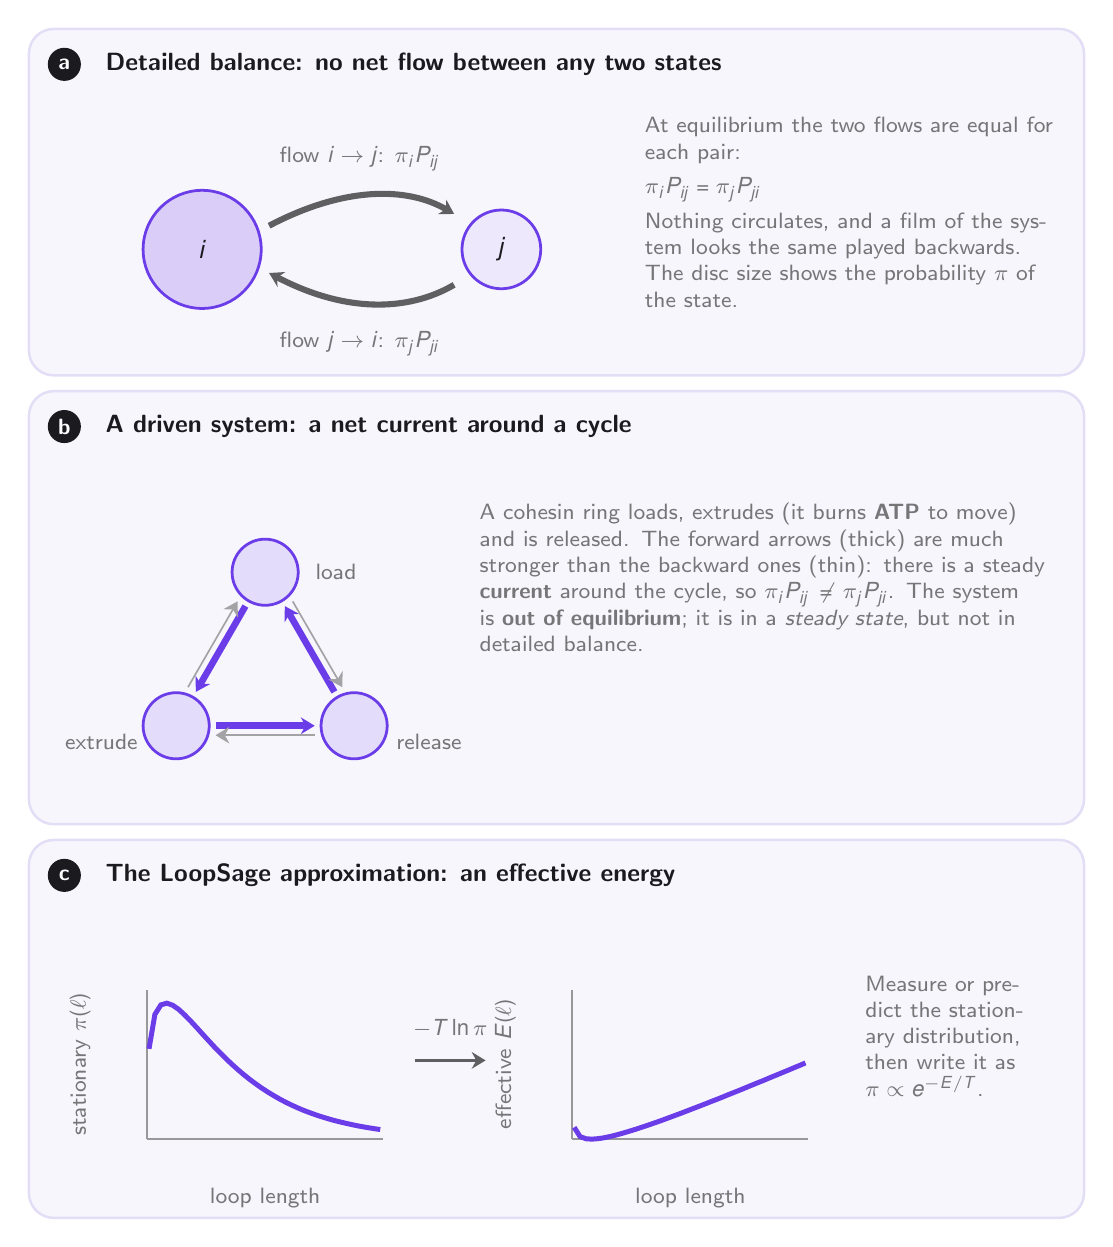
\begin{tikzpicture}
  \panelbg{0}{9.0}{13.4}{13.4}\badge{0.45}{12.950000000000001}{a}\node[hd] at (0.85,12.950000000000001) {Detailed balance: no net flow between any two states};
  \panelbg{0}{3.3}{13.4}{8.8}\badge{0.45}{8.350000000000001}{b}\node[hd] at (0.85,8.350000000000001) {A driven system: a net current around a cycle};
  \panelbg{0}{-1.7}{13.4}{3.1}\badge{0.45}{2.65}{c}\node[hd] at (0.85,2.65) {The LoopSage approximation: an effective energy};
  \fill[cohesin!25] (2.2,10.6) circle (0.75);\draw[cohesin,line width=1pt] (2.2,10.6) circle (0.75);\node[lab] at (2.2,10.6) {$i$};
  \fill[cohesin!12] (6.0,10.6) circle (0.5);\draw[cohesin,line width=1pt] (6.0,10.6) circle (0.5);\node[lab] at (6.0,10.6) {$j$};
  \draw[mv,line width=2.2pt] (3.05,10.9) .. controls (4.0,11.4) and (4.8,11.4) .. (5.4,11.05);
  \draw[mv,line width=2.2pt] (5.4,10.15) .. controls (4.8,9.8) and (4.0,9.8) .. (3.05,10.3);
  \node[note] at (4.2,11.75) {flow $i\to j$: $\pi_i P_{ij}$};\node[note] at (4.2,9.4) {flow $j\to i$: $\pi_j P_{ji}$};
  \node[note,text width=5.3cm,anchor=north west] at (7.7,12.4) {At equilibrium the two flows are equal for each pair:\\[3pt]$\pi_i P_{ij}=\pi_j P_{ji}$\\[3pt]Nothing circulates, and a film of the system looks the same played backwards. The disc size shows the probability $\pi$ of the state.};
  \fill[cohesin!18] (3.00,6.50) circle (0.42);\draw[cohesin,line width=1pt] (3.00,6.50) circle (0.42);
  \fill[cohesin!18] (1.87,4.55) circle (0.42);\draw[cohesin,line width=1pt] (1.87,4.55) circle (0.42);
  \fill[cohesin!18] (4.13,4.55) circle (0.42);\draw[cohesin,line width=1pt] (4.13,4.55) circle (0.42);
  \draw[mv,line width=2.4pt,cohesin] (2.75,6.07)--(2.12,4.98);
  \draw[mv,line width=0.6pt,ink!40] (2.02,5.04)--(2.65,6.13);
  \draw[mv,line width=2.4pt,cohesin] (2.37,4.55)--(3.63,4.55);
  \draw[mv,line width=0.6pt,ink!40] (3.63,4.43)--(2.37,4.43);
  \draw[mv,line width=2.4pt,cohesin] (3.88,4.98)--(3.25,6.07);
  \draw[mv,line width=0.6pt,ink!40] (3.35,6.13)--(3.98,5.04);
  \node[note] at (3.90,6.50) {load};\node[note] at (0.92,4.35) {extrude};\node[note] at (5.08,4.35) {release};
  \node[note,text width=7.2cm,anchor=north west] at (5.6,7.5) {A cohesin ring loads, extrudes (it burns \textbf{ATP} to move) and is released. The forward arrows (thick) are much stronger than the backward ones (thin): there is a steady \textbf{current} around the cycle, so $\pi_iP_{ij}\neq\pi_jP_{ji}$. The system is \textbf{out of equilibrium}; it is in a \emph{steady state}, but not in detailed balance.};
  \draw[ln] (1.5,-0.7)--(4.5,-0.7);\draw[ln] (1.5,-0.7)--(1.5,1.2);
  \node[note] at (3.00,-1.45) {loop length};
  \node[note,rotate=90] at (0.65,0.25) {stationary $\pi(\ell)$};
  \draw[cur] plot coordinates {(1.525,0.447) (1.600,0.884) (1.676,1.005) (1.751,1.027) (1.826,1.001) (1.902,0.948) (1.977,0.879) (2.052,0.802) (2.128,0.720) (2.203,0.637) (2.278,0.555) (2.353,0.474) (2.429,0.396) (2.504,0.321) (2.579,0.250) (2.655,0.182) (2.730,0.118) (2.805,0.058) (2.881,0.002) (2.956,-0.051) (3.031,-0.100) (3.107,-0.146) (3.182,-0.189) (3.257,-0.229) (3.333,-0.266) (3.408,-0.300) (3.483,-0.332) (3.559,-0.361) (3.634,-0.388) (3.709,-0.413) (3.784,-0.436) (3.860,-0.458) (3.935,-0.477) (4.010,-0.495) (4.086,-0.512) (4.161,-0.528) (4.236,-0.542) (4.312,-0.555) (4.387,-0.567) (4.462,-0.578)};
  \draw[ln] (6.9,-0.7)--(9.9,-0.7);\draw[ln] (6.9,-0.7)--(6.9,1.2);
  \node[note] at (8.40,-1.45) {loop length};
  \node[note,rotate=90] at (6.05,0.25) {effective $E(\ell)$};
  \draw[cur] plot coordinates {(6.925,-0.550) (7.000,-0.668) (7.076,-0.695) (7.151,-0.700) (7.226,-0.694) (7.302,-0.683) (7.377,-0.667) (7.452,-0.649) (7.528,-0.628) (7.603,-0.606) (7.678,-0.583) (7.753,-0.559) (7.829,-0.534) (7.904,-0.508) (7.979,-0.482) (8.055,-0.455) (8.130,-0.427) (8.205,-0.399) (8.281,-0.371) (8.356,-0.342) (8.431,-0.313) (8.507,-0.284) (8.582,-0.255) (8.657,-0.225) (8.733,-0.196) (8.808,-0.166) (8.883,-0.135) (8.959,-0.105) (9.034,-0.075) (9.109,-0.044) (9.184,-0.013) (9.260,0.018) (9.335,0.048) (9.410,0.080) (9.486,0.111) (9.561,0.142) (9.636,0.173) (9.712,0.205) (9.787,0.236) (9.862,0.268)};
  \draw[mv] (4.9,0.3)--(5.8,0.3);\node[note] at (5.35,0.7) {$-T\ln\pi$};
  \node[note,text width=2.5cm,anchor=north west] at (10.5,1.5) {Measure or predict the stationary distribution, then write it as $\pi\propto e^{-E/T}$.};
\end{tikzpicture}
\end{document}
